%%========================================================================
%% LaTeX sjabloon voor stage/projectrapport of bachelorproef
%%  HoGent Bedrijf en Organisatie
%%========================================================================

%%========================================================================
%% Preamble
%%========================================================================

\documentclass[pdftex,a4paper,12pt,twoside]{report}

% XXX: Let op: dit sjabloon is gemaakt om dubbelzijdig af te drukken
% Voor enkelzijdig, verwijder ``twoside'' hierboven.

%%---------- Extra functionaliteit ---------------------------------------

\usepackage[utf8]{inputenc}  % Accenten gebruiken in tekst (vb. é ipv \'e)
\usepackage{amsfonts}        % AMS math packages: extra wiskundige
\usepackage{amsmath}         %   symbolen (o.a. getallen-
\usepackage{amssymb}         %   verzamelingen N, R, Z, Q, etc.)
\usepackage[english]{babel}    % Taalinstellingen: woordsplitsingen,
                             %  commando's voor speciale karakters
                             %  ("english" voor EN)
\usepackage{eurosym}         % Euro-symbool €
\usepackage{geometry}
\usepackage{graphicx}        % Invoegen van tekeningen
\usepackage[pdftex,bookmarks=true]{hyperref}
                             % PDF krijgt klikbare links & verwijzingen,
                             %  inhoudstafel
\usepackage{listings}        % Broncode mooi opmaken
\usepackage{multirow}        % Tekst over verschillende cellen in tabellen
\usepackage{rotating}        % Tabellen en figuren roteren
\usepackage{natbib}          % Betere bibliografiestijlen
\usepackage{fancyhdr}        % Pagina-opmaak met hoofd- en voettekst

\usepackage[T1]{fontenc}     % Ivm lettertypes
\usepackage{lmodern}
\usepackage{textcomp}

\usepackage{lipsum}          % Voor vultekst (lorem ipsum)

%%---------- Layout ------------------------------------------------------

% hoofdingen, enz.
\pagestyle{fancy}
% enkel hoofdstuktitel in hoofding, geen sectietitel (vermijd overlap)
\renewcommand{\sectionmark}[1]{}

% lijn, wordt gebruikt in titelpagina
\newcommand{\HRule}{\rule{\linewidth}{0.5mm}}

% Leeg blad
\newcommand{\emptypage}{
\newpage
\thispagestyle{empty}
\mbox{}
\newpage
}

% Gebruik een schreefloos lettertype ipv het "oubollig" uitziende
% Computer Modern
\renewcommand{\familydefault}{\sfdefault}

% Commando voor invoegen Java-broncodebestanden (dank aan Niels Corneille)
% Gebruik: \codefragment{source/MijnKlasse.java}{Uitleg bij de code}
\newcommand{\codefragment}[2]{ \lstset{%
  language=java,
  breaklines=true,
  float=th,
  caption={#2},
  basicstyle=\scriptsize,
  frame=single,
  extendedchars=\true
}
\lstinputlisting{#1}}

%%---------- Documenteigenschappen ---------------------------------------
%% Vul dit aan met je eigen info:

% Je eigen naam
\newcommand{\student}{Frederik De Smedt}

% De naam van je lector, begeleider, promotor
\newcommand{\promotor}{Joeri Van Herreweghe}

% De naam van je co-promotor
\newcommand{\copromotor}{Jens Buysse}

% Indien je bachelorproef in opdracht van een bedrijf of organisatie
% geschreven is, geef je hier de naam.
\newcommand{\instelling}{---}

% De titel van het rapport/bachelorproef
\newcommand{\titel}{Research of caching strategies in mobile native applications using external data services}

% Datum van indienen
\newcommand{\datum}{29 mei 2015}

% Faculteit
\newcommand{\faculteit}{Faculteit Bedrijf en Organisatie}

% Soort rapport
\newcommand{\rapporttype}{Scriptie voorgedragen tot het bekomen van de graad van\\Bachelor in de toegepaste informatica}

% Academiejaar
\newcommand{\academiejaar}{2015-2016}

% Examenperiode
%  - 1e semester = 1e examenperiode
%  - 2e semester = 2e examenperiode
%  - tweede zit = 3e examenperiode
\newcommand{\examenperiode}{Tweede examenperiode}

%%========================================================================
%% Inhoud document
%%========================================================================

\begin{document}

%%---------- Front matter ------------------------------------------------
%% Het voorblad - Hier moet je in principe niets wijzigen.

\begin{titlepage}
  \newgeometry{top=2cm,bottom=1.5cm,left=1.5cm,right=1.5cm}
  \begin{center}

    \begingroup
    \rmfamily
    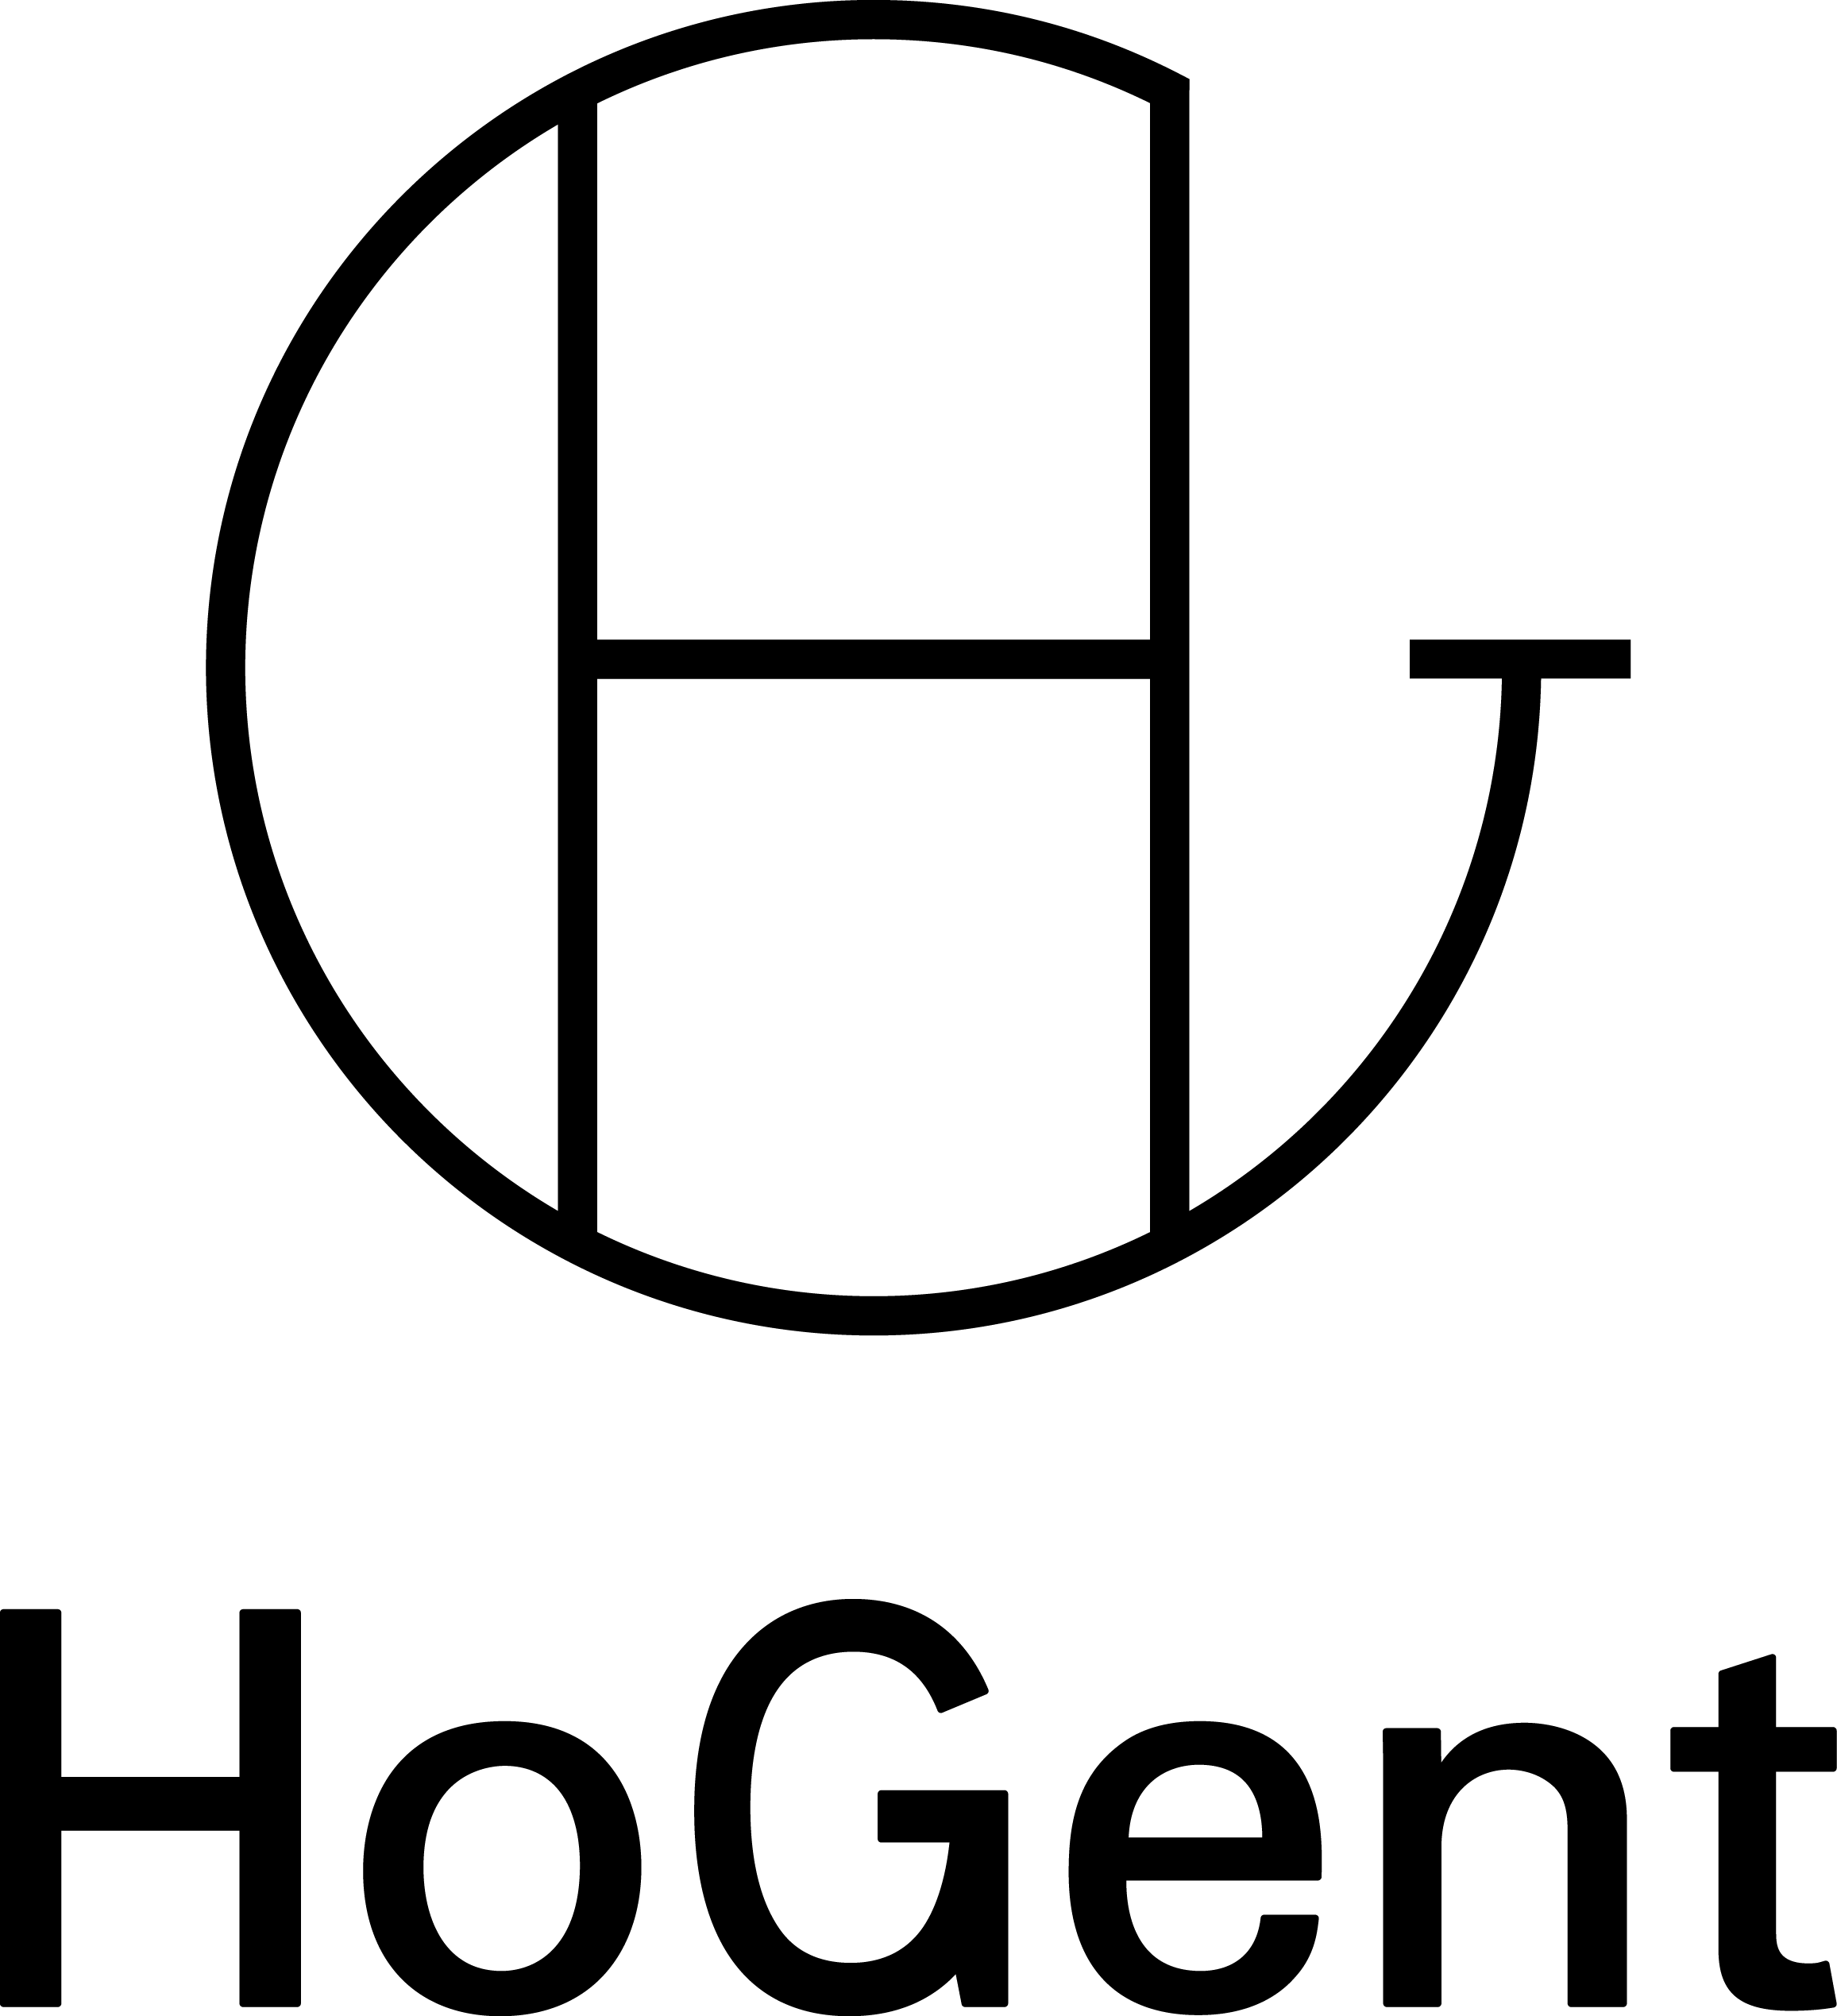
\includegraphics[width=2.5cm]{img/HG-beeldmerk-woordmerk}\\[.5cm]
    \faculteit\\[3cm]
    \titel
    \vfill
    \student\\[3.5cm]
    \rapporttype\\[2cm]
    Promotor:\\
    \promotor\\
    Co-promotor:\\
    \copromotor\\[2.5cm]
    Instelling: \instelling\\[.5cm]
    Academiejaar: \academiejaar\\[.5cm]
    \examenperiode
    \endgroup

  \end{center}
  \restoregeometry
\end{titlepage}

% Schutblad

\emptypage


\begin{titlepage}
  \newgeometry{top=5.35cm,bottom=1.5cm,left=1.5cm,right=1.5cm}
  \begin{center}

    \begingroup
    \rmfamily
    \faculteit\\[3cm]
    \titel
    \vfill
    \student\\[3.5cm]
    \rapporttype\\[2cm]
    Promotor:\\
    \promotor\\
    Co-promotor:\\
    \copromotor\\[2.5cm]
    Instelling: \instelling\\[.5cm]
    Academiejaar: \academiejaar\\[.5cm]
    \examenperiode
    \endgroup

  \end{center}
  \restoregeometry
\end{titlepage}


\begin{abstract}
% TODO: De "abstract" of samenvatting is een kernachtige (max 1 blz. voor een
% thesis) synthese van het document. In ons geval beschrijf je kort de
% probleemstelling en de context, de onderzoeksvragen, de aanpak en de
% resultaten.
  \lipsum[1-4]
\end{abstract}

\chapter*{Voorwoord}
\label{ch:voorwoord}

% TODO: Vergeet ook niet te bedanken wie je geholpen/gesteund/... heeft
\lipsum[5-6]

\tableofcontents

% Als je een lijst van afkortingen of termen wil toevoegen, dan hoort die
% hier thuis. Gebruik bijvoorbeeld de ``glossaries'' package.

%%---------- Kern --------------------------------------------------------

\chapter{Introduction}
\label{ch:introduction}
The definition of mobile has changed a lot in the last few years and the expectations of mobile applications continue to rise.
Mobile applications should work on a myriad of devices and screen resolutions, and should take battery efficiency into account.
Furthermore is an application no longer really considered mobile if it isn't available without a stable internet connection.
This makes research about caching in mobile applications really interesting since it can solve multiple problems.
Caching of the results of expensive operations, e.g. an internet connection, will allow the system to avoid many of these operations,
reducing battery consumption, and can these results be used when a (temporary) connection loss would occur.
\\\\
Lots of IT companies already implement such a system:
\begin{itemize}
\item The Facebook-app still shows several posts and pictures when you have no internet connection;
\item Third-party API's, such as Picasso (Android) and SDWebImage (iOS) retrieve images from the web and have an embedded caching system;
\item Twitter allows you to change account settings offline, which are later synchronized with the backend when a connection is established\footnotemark.
\end{itemize}
\footnotetext{In this example we are talking more about persistent data, however it is used to store temporary data that can later be forgotten once it is synchronized with the backend. Just like a cache containing business data.}
\newpage
\section{Problem definition and research questions}
However mobile caching is becoming more and more common, there is no real framework on which they all rely. Instead they each have to think about how to implement
caching and have to invest in discovering caching strategies and inventing a good caching implementation.
\\\\
They can decide to ignore the caching problem and focus on the business logic and the actual functional requirements of the project. The chances that the
project is able to be completed within the deadline increases, as they have less work to do. However, if there is a non-functional requirement that requires some sort of caching
or if the users of the application are complaining about problems that come along (e.g. lots of traffic or battery usage), you will have to implement the caching system afterwards. Which might force them to redesign parts of the system (both frontend and backend) or forces you to do this in an incomplete way, introducing lots of bugs that usually come along in caching systems.
\label{sec:research questions}
Every platform already has some infrastructure designed to allow caching, e.g. Guava and a local lightweight database.
Yet there is more to caching than simply storing information, developers should think about what data is eligible for caching and how this can improve their application.
They should be able to do this with an efficient method, customized to the needs of the application considering all possible events that might occur and how they might be able to handle this. These ideas and strategies should then be implemented in both the backend and frontend, however the backend implementation could be reduced to an almost non-existing implementation, since it is not merely about the native application itself, but about the data flow between the different systems.
\\\\Because of these reasons, we will try to answer the following questions in this article:
\begin{itemize}
\item How can a caching strategy efficiently store and fetch data in a native mobile application?
\item What life-cycle events should be considered and how can they react to these events?
\item How can the cache be synchronized with the external data service (backend)?
\end{itemize}
\chapter{Methodology}
\label{ch:methodology}
First, a literature study will take place about caching in general: what concepts and principles are used? Which steps can be differentiated when interacting with a cache? What are some common techniques? Some of these will later be revisited and possibly simplified, to use them on a mobile device.
\\\\
At the same time, research can be done defining which events are commonly handled by a mobile native application. However the case study will be performed in the Android platform, it is important to consider all platforms (Android, iOS, Windows) and how each of them handles these events.
\\\\
After these first two steps, we can think about how the cache could respond to these different events and why and when this would be beneficial. Depending on the needs of the cache, the ultimate result should maintain the caches integrity, especially concerning business data. Possibly critical business data could be lost or even worse: wrong or insufficient business data could later be synchronized to and from the underlying data service.
\\\\
Parallel with step 3, a literatur study concerning the synchronization between the frontend cache and the underlying data service will be done. What techniques are commonly used? What happens when there is two-way synchronization and there is conflicting data? Although this is partially out of the scope of the frontend developer, it is important that everyone has a clear view of what they can do to facilitate synchronization. The backend can influence frontend performance and the frontend can influence backend performance!
\\\\
All these concepts and ideas will then be tested in a case study, which will analyze the performance, from an frontend Android application and a backend Java EE application. 
When talking about performance, this will be mainly about the performance benefits on the frontend. Performance benefits of caching in the backend is not in the scope of this thesis.
% TODO: Hoe ben je te werk gegaan? Verdeel je onderzoek in grote fasen, en
% licht in elke fase toe welke stappen je gevolgd hebt. Verantwoord waarom je
% op deze manier te werk gegaan bent. Je moet kunnen aantonen dat je de best
% mogelijke manier toegepast hebt om een antwoord te vinden op de
% onderzoeksvraag.

\chapter{Basics of caching}
\label{ch:caching}
A cache can be defined as a (fast) memory structure designed to reduce costs and improve speeds of computer operations.
The term caching is widely used in computer science, from the CPU that uses different multi-level caches, to web caches concerning
the reuse of already fetched HTTP pages \citep{rfc2616} and all of them are designed to improve performance. Even low-end devices such as microcontrollers
can benefit on the usage of a cache \citep{extremetech_multilevelcache}. How this memory structure improves the performance
is dependent on the use case in which it used. It could keep the results of long operations or use tokens to check whether data is outdated.
\section{Basic cache performance metrics}
The presence of a cache by itself will not cause a performance increase. It is integrated in a software application that uses a cache. The application then checks whether certain data is present in the cache and if not, does everything it needs to do in order to retrieve this data from a third party. In most examples a cache can be represented by a collection of key/value pairs, to which the application requests a value based on a key. When the cache contains the data the application is requesting, it is commonly known as a \emph{cache hit}. Inversely, when the cache does not contain the requested data, it is known as a \emph{cache miss}. The relationship between the total amount of requests and the total amount of hits is the \emph{hit ratio}.
$R=h/n$ where $R$ is the hit ratio, $h$ is the total amount of cache hits and $n$ is the amount of cache requests.
These terms are, among others, important factors determining the performance of a cache. A common misconception is that a high hit ratio results in better cache performance, yet this is only true considering hit ratios. If the hit ratio were the only factor, the caches ``performance'' would be proportional to the size of the cache and a cache of 10Tb always yield better performance than a cache of 20Mb \citep{wulf1995hitting}. This statement can easily be proven wrong when considering other factors such as speed, as the 20Mb cache will need far less time to produce a result than the cache of 10Tb.
\section{Paging}
However caching is of high importance with lots of aspects in IT, caching is what it is today thanks to some specific problems that have received lots of attentions the last decades. Perhaps the most important problem, considering the field of caching, is the problem with \emph{virtual memory} \citep{denning1970virtual}. Virtual memory maps virtual memory addresses, provided by an operating system to a program, to actual hardware memory addresses. This way, the operating system can manage its memory resources and decide where to store and retrieve data from programs using virtual memory. This was considered a very elegant way to increase programming productivity, as programmers could use a high-level API to retrieve and store data instead of needing to talk directly to the processor, which would also make them machine dependent.
\\\\
The operating system can assign priorities to memory addresses and decide whether it should be stored on a fast or slow memory. The memory of an idle process could for example be persisted on slow memory, i.e. hard drive, so that the faster memory, i.e. RAM, can be used for memory of currently active processes. The moment that the idle process wakes up, it can still use the virtual memory pointers, as if the data has never moved. When a process tries to access a piece of data, currently stored on the hard drive, the operating system will produce a \emph{page fault}. This event will cause the \emph{page}, a block of data, containing the desired data on the hard drive to be transfered to somewhere in RAM memory.
\\\\
The memory transfer due to a page fault is however very expensive as the hard drive is a lot slower than RAM memory and the processor itself. Therefore it is important to have a good paging strategy, an algorithm that decides which pages will be persisted to the hard drive and which pages will remain in RAM memory. The optimal algorithm will only persist the pages that will not be used for the longest period of time.
\\\\
The paging problem is very similar to finding the optimal caching strategy, RAM memory is the cache, the hard drive is non-cached memory and we are looking for an algorithm such that only the least interesting memory is removed from the cache. The principle ultimately solving the paging problem is therefore one of the fundamental principles not only in pages and virtual memory, but all of caching, this principle is called the \emph{locality principle}.
\\\\
\section{Locality principle}
\subsection{What is the locality principle}
When people are executing a process, such as preparing dinner, they always tend to gather everything they need before or during the process. If it were a bigger meal the entire meal is divided in a set of subprocesses. When preparing lasagne it could be divided in preparing the tomato sauce, creating each layer using previously prepared ingredients, etc. The principle of dividing a large task in a set of smaller subtasks is called \emph{divide and conquer}. % TODO: Find reference for divide and conquer
When creating the lasagne layers, we would first collect all supplies needed (tomato sauce, lasagne sheets, etc) and put them somewhere close, e.g. on the counter, once that is done, the layers are assembled. This is more practical and time saving than to continually walk a relatively long distance each time you need the tomato sauce.
\\\\
Something similar has been discovered with programs by \cite{locality_principle} when analyzing memory usage of multiprogramming systems using virtual memory in 1967.
He formalized this idea through the years and called it the \emph{locality principle} also commonly known as \emph{locality of reference}. He found that programs intrinsically use a very small part of data when performing arbitrary algorithms. In 1980 he formally defined a relationship between the processor, executing the instructions, and the data/object it uses called the \emph{distance} and is denoted as $D(x,t)$ where x is the object and t is the current time. The relevance of this object to the processor at a certain time is based on whether the distance is less than a certain threshold:
\[
	D(x,t) \leq T
\]
where T is the threshold and D(x,t) is the distance function. The threshold and the distance are embedded in a, usually 2 dimensional, spatial-temporal coordinate space where the spatial dimension is the memory address of the object and the temporal dimension is the time when it was accessed.

\subsection{Interpreting spatial-temporal distances}
Because the distance function $D$ is operating in a spatial-temporal space, it is based on the definition and interpretation of the two different dimensions.
The easiest way to understand how these dimensions can be interpreted is to look at them seperately. Once that is understood, you simply need a function 
$m : S \times T \to \Theta$ where $S$ is the set representing the spatial dimension, $T$ is the set representing the temporal dimension and $\Theta$ is the set representing the spatial-temporal space.
\newpage
\emph{Temporal distance}, the distance in time that can be expressed in several ways:
\begin{itemize}
\item time since last reference
\item time until next reference
\item access time to get the object
\item a combination of the above or others
\end{itemize}
The time since the last reference to object $x$ can be known by storing the references used by the processor and the time when the reference happened in a list. The time until next reference might yield better results when trying to create an effective and efficient cache since it is known when the object will be used again. However this should require a learning agent that can try and calculate when the next reference will happen based on the reference history. The time unit used should be a relative unit such as the execution of an instruction, this is better than an absolute unit such as seconds because it will ignore external factors that shouldn't affect the distance, e.g. other processes running.
\\\\
\emph{Spatial distance}, the distance to the location of the object can be expressed in several ways as well:
\begin{itemize}
\item the amount of hops in a network required to retrieve the contents
\item the memory on which the data is stored, e.g. objects stored in RAM have a smaller spatial distance than objects stored on a hard drive
\item the number of memory addresses between the object and the addresses currently being used or pointed to
\item a combination of the above or others
\end{itemize}
Intuitively, one could see a relationship between the spatial and temporal locality. When the spatial distance to an object is greater, the temporal distance usually also increases because it will need to cover more ground to retrieve the object. When the temporal distance is greater the spatial distance will usually increase because of pacification of the object: it will be stored on slower memory due to the lack of interaction.
When checking the relevance of objects to the processor are checked, with $D(x,t) \leq T$, only some objects will pass the inequality, the set of these objects is 
called the \emph{working set}. It are the objects in the working set that would, among others, be candidates for caching. 
\section{CRUD}
When interacting with a cache, there are, in general, several operations that each cache is able to do. In general, you will want all operations that allow you to read the contents of a cache and to get from an arbitrary cache state, to any other arbitrary cache state through, possibly composite, operations. These operations are known as CRUD operations and are a main part of RESTful web services \citep{battle2008bridging}. This will allow an easier implementation when using Read Through (or Cache Aside) Caches.
% TODO: Add reference to section about read through and cache aside
\emph{CRUD} is an acronym for Create Read Update Delete and as the name suggests, 4 operations can be distinguished:
\begin{itemize}
\item \emph{Create} allows some client to add an object to a data set. When adding an object to a cache you will typically invoke an add-function receiving two arguments: a key and a value. SQL implements this with its INSERT-statements and HTTP integrates this using a POST request.
\item \emph{Read} is used to get all information or a subset of information from a data set, in a typical cache this will be integrated as a get-function receiving
the key of the value you wish to access. \emph{The key passed to the function is the same key that is passed to the add-function when creating a new cache entry.} SQL implements this with its SELECT-statements, commonly known as queries, and HTTP integrates this using a GET request.
\item \emph{Update} will change the contents of an existing object, this is separated from Create as these two might be treated differently, depending on the system in which the data set is embedded. A cache will mostly provide a common API for both Create and Update: a function with a key and a value as its parameters. Yet they might be seperated into separate functions to increase readability or to simplify event triggering. SQL implements this with its UPDATE-statement and HTTP implements this using PUT-requests.
\item \emph{Delete} is used when an element should no longer be an element of the data set. In a cache this might happen when an object is outdated, or if the object has also been removed in the data service. You would then call a delete-function passing the key of the object that should be removed. SQL implements this with its DELETE-statements and HTTP integrates this with its DELETE request.
\end{itemize}
\citep{battle2008bridging} Note how these operations are defined on the database-level, software application level, and networking level. Also note how an interface of a cache should at least contain functions allowing the user to execute all CRUD-operations, yet they are not limited by them.
\chapter{Cache replacement algorithms}
Now that we know \emph{what} should be possible with caches, we can ask ourselves the question \emph{how} we could implement all of this, the algorithms implementing a cache system are called \emph{cache replacement algorithms} or \emph{cache replacement policies}. Yet not just any cache replacement algorithm will do, we are trying to find the most optimal algorithm, the one that will provide the best (performance) results by interacting with it using CRUD-operations. 
Although most algorithms are only based on your interactions with the cache, some algorithms can be run on separate processes/threads that are
then responsible for maintaining the cache even without interactions with the user.
\section{RR}
The first cache replacement algorithm that will be discussed is the Random Replacement strategy. Of all the strategies, this one could be considered one of the strategies with the lowest overhead and the easiest implementations \citep{random_replacement}. This makes it ideal for certain low-level systems or hardware that cannot afford many processing cycles on cache management.
\paragraph{Read} When trying to get a certain object by its key, the algorithm can use any sorted or non-sorted collection. When using an non-sorted collection it would check each element in the collection in $\mathcal{O}(n)$. Note how this defines the upper bound of the function, therefore it could also be in constant time or $\mathcal{O}(\log_2n)$ when performing a binary search on a sorted list.
\paragraph{Create} When adding an object while the cache is not yet full, it could simply be added to the collection, algorithm-independently. When the cache is already full, the algorithm will randomly remove replace an object from the collection by the new object that should be stored. The operation itself is primitive and easy to program, the only difficulty is creating a reliable random generator, yet this is not in the scope of this algorithm.
\paragraph{Update} Updating is similar to \emph{create}, if the key is present it will result in a \emph{read} to get the appropriate object and then changes the object. If the key is not in the cache, it could either \emph{create} object or alarm the user that it is not present.
\paragraph{Delete} When deleting an object, based on a key, it can be done by first performing a \emph{read} to know whether the key is present and if so removing it. Yet some collections will do this nevertheless, in that scenario the algorithm could simply delegate to the delete function from the backing collection.
\section{FIFO}
FIFO, acronym for First-In-First-Out, is a cache replacement policy much like a queue. New objects are inserted at one end of the queue, when the cache is full the first object at the other end will be discarded and the new object will be added at the insertion end \citep{reineke2007timing}. FIFO is analogous to FCFS, First-Come First-Served, which is used in OS scheduling algorithms.
Note that the hit ratio performance of the FIFO replacement strategy is like the hit ratio performance of the RR replacement strategy \citep{rao1978performance}.
\paragraph{Read} A read in a FIFO policy results in a queue being scanned in $\Theta(n)$, almost just like RR. The difference between RR and FIFO is that a FIFO cannot be a sorted collection, since its performance is based on a ``constantly'' defined sorting structure, this means that you cannot just swap two elements in the cache and expect it to work just the same: you have changed the actual state of the cache. Just like RR, a read does not change the state of the cache.
\paragraph{Create} When adding a new object to the cache it will, without loss of generality, be placed on the left side of the queue. When the queue is full, the first element on the right will be removed and all other objects will be ``moved to the right'' (however this is not an actual operation that occurs in an efficient queue implementation), clearing a space on the left, ready to be filled in by the new object.
\paragraph{Update} When updating an existing object, based on a key, there will be a read that will then change the object at the index $i$ by the new object. After the object $x$ is updated, $x$ should then be removed from the queue, every element left of $x$ should then be moved to the right and $x$ is again added to the left side of the queue. Note that all these operations should be executed in a procedural or atomic way.
\paragraph{Delete} When deleting an existing object, you scan the queue until you find the index with value $x$ corresponding to the given key. You will then remove $x$ and move all elements left of $x$ to the right. The next object added to the queue will therefore not cause the object (completely) at the right to be removed from the cache.
\section{LRU}
An \emph{LRU}-cache (Least Recently Used Cache) is possibly the most popular and one of the best cache replacement algorithms out there. There are lots of variants on LRU and therefore it can also be seen as a cache replacement algorithm family. The probability of an object being present in a cache, the hit rate $h(n)$, can be approximated by 
$h(n) \approx 1 - e^{-q(n)t_C}$, where $n$ is the object being requested, $q(n)$ is the popularity of the object (see \emph{Zipf's law}) and $t_C$ being the (unique) root of 
$\sum_{n=1}^N(1-e^{-q(n)t})=C$, with $N$ being the maximum amount of objects in the cache and $C$ the cache capacity. This approximation is called the \emph{Che approximation} \citep{fricker2012versatile}.
\\\\
The LRU algorithm is all about replacing the least recently used object, in other words, when a new object should be added to a full cache, it will remove the object that hasn't been accessed for the longest period of time. To know when an object has last been accessed, the usual implementation uses a map, let's call it the \emph{key history map} that can get a timestamp (this can be in milliseconds or can be some relative time unit) based on a key. However it could also be implemented by a queue, where the order of the queue determines which objects have, relatively, been accessed most recently.
\paragraph{Read} Retrieving an object based on a key, first boils down to retrieving a value from any collection, just like RR. When the object is found it will not immediately return this, yet it will firstly access the \emph{key history map} and update the timestamp to its newest value. This way the algorithm will know, in the future, that this key has just been accessed. If the LRU is implemented using a queue, it will, without loss of generality, remove the object $x$ at index $i$, (conceptually) move all objects left of $i$ to the right (which is equivalent to incrementing the index $j$ of all objects where $j < i$) and $x$ will then be inserted at the left side of the queue.
\paragraph{Create} If the cache is not yet full, the object will be added to the collection and the key history map will be updated with a new timestamp for the specified key. If the cache is full, it will first find the key with the lowest timestamp, which is the object that hasn't been accessed for the longest period of time (considering an increasing time function). It will then remove this key in the collection and remove the corresponding key from the map, the object will then be added to the collection and the key history map will be updated with a new timestamp for the specified key. When using a queue with a cache that is not yet full, you will add the new object, without loss of generality, to the left side of the queue. When using a queue with a full cache, you will remove the object to the right of the queue, move all remaining objects to the right, and then add the new object to the left of the queue.
\paragraph{Update} The algorithm will check if the key is already stored in the collection, if not, this boils down to \emph{creating} (adding) a new object to the collection or queue. When the key is stored in the cache, it will update the object in the collection to the new object and then it will update the timestamp of the corresponding key in the key history map. When using a queue, it will remove the object with the specified key from the queue, move all objects to the left of the object to the right, and then add the new object, without loss of generality, to the left side of the queue.
\paragraph{Delete} To remove an object from the cache, the object is simply removed from both the collection and the key history map. When using a queue, it will remove the object $x$ from the queue and move all objects left of $x$ to the right.
\\\\
\citep{lru_implementation}This is the basic implementation of an LRU cache, yet there are lots of variants. There are algorithms taking a new approach, based on LRU, there are some algorithms that have a highly specialized implementation of LRU, and there are even some implementations that use LRU together with some other cache replacement algorithm to try and get optimal results based on the situation it is in.
\section{MRU}
The next algorithm is very similar to LRU, \emph{MRU} is an acronym for \emph{Most Recently Used} and will evict the most recently accessed objects when adding a new object to an already full cache. LRU and MRU should not be seen as ``competitors'' of each other, but rather a twin where, most of the time, one of the two can be chosen based on the context.
If it makes sense that a recently requested object has a high probability of being requested again in the near future, you can use LRU. If it makes more sense that a recently requested object will not be requested any time soon, you can choose an MRU cache replacement strategy. Even though one would think LRU would be used most of the time, there are abundant scenario's where MRU would make a lot of sense also. Consider a cache containing Facebook-posts, would it work better under an MRU or an LRU system? To answer this question further research should be done, but MRU makes a very good candidate, considering people tend not to revisit posts they have just visited 10 minutes earlier. If the user were to respond or like the post, he could however receive notifications of new people posting comments and thus LRU could be more useful.
\paragraph{Read} Every object in the cache stores an extra bit (or boolean) called the MRU-bit and is used to find out whether the object has recently been visited, let's
say that every object in the cache is stored as a tupel $(b,x)$, where $b$ is the MRU-bit and $x$ is the actual object stored. First the algorithm will check if the object is present in the cache and if so, we'll call the index $i$ and it will set $b$ to 1 or true. This is used to indicate that it has just been accessed. Next the algorithm will check if there exists another index where the MRU-bit is not 1, if so the algorithm ends, otherwise it will flip the MRU-bit at every index back to 0 or false, this is called a 
\emph{global-flip}. This is the same as checking if $\exists i \in I : B(i) = 0$, where $I$ is the collection of all indexes and $B : I \to \{0,1\}$ is the function that gets the MRU-bit of the object at an index. This can be refactored as $\forall i \in I : B(i) = 1$, so checking for the existence of an index with an MRU-bit at 0 or false is the same as checking whether every MRU-bit is 1 or true.
\paragraph{Create} When the cache is not yet full, the next object will be added to the end of the cache and its MRU-bit will directly be set to 1 or true (ensuring it will not 
be replaced before the next \emph{global-flip}. If the cache is full it will look for an index $j$, such that $B(j) = 0$ and $\forall i \in I : i < j, B(i) = 0$, so $j$ is the first index with a 0 or false MRU-bit. Note that there will \emph{always} be at least 1 index with a 0 or false MRU-bit due to global-flipping.
\paragraph{Update} If the object is not yet present in the cache, it will delegate the object to \emph{create}. If it is in the cache, it will replace the object, while keeping it at the same position, and set its MRU-bit to 1 or true. If the MRU-bit was previously 0 or false, it is important to check if a \emph{global-flip} should be executed or not. Yet it is always safe to check for this, even if the MRU-bit hasn't changed (and already was on 1 or true).
\paragraph{Delete} To remove an object, you first check whether the object is present in the cache, if it is not then you don't have to do anything, if it is present at index $i$, you move the object at every index $j$ such that $j > i$ to the left which is the same as decrementing $j$ by one, so $j \leftarrow j - 1$.
\citep{guan2014wcet}
\section{LFU}
\section{LIRS?}
\section{Bélády's algorithm}
There is currently no \emph{trivial} cache mechanism focusing on spatial locality, this would be a cache keeping objects predicted to be accessed due to some spatial locality/localities. \emph{Bélády's algorithm} is considered the most optimal cache replacement algorithm available, as it discards the objects from which he knows it will not be needed for the longest period of time \citep{cache-algorithm-lru-belady}. Yet there are no claims whether this is the most optimal cache replacement algorithm considering a dynamic cost for retrieving uncached data.

% TODO: Talk about how the algorithms are storing simply ``an object'', yet this is usually a key-value pair
% TODO: Talk about how we are not talking about what happens if the cache does not find the object (cache aside & read through)
% TODO: Read file:///D:/School/TI-3AS2/Bachelorproef/Bronnen/1-s2.0-S0140366400003121-main.pdf

\chapter{Conclusion}
\label{ch:conclusion}

% TODO: Trek een duidelijke conclusie, in de vorm van een antwoord op de
% onderzoeksvra(a)g(en). Reflecteer kritisch over het resultaat. Zijn er
% zaken die nog niet duidelijk zijn? Heeft het ondezoek geleid tot nieuwe
% vragen die uitnodigen tot verder onderzoek?
\lipsum[76-80]


\bibliographystyle{apa}
\bibliography{tin-bachproef}

%%---------- Back matter -------------------------------------------------

\listoffigures
\listoftables

\end{document}
